\documentclass[11pt]{scrartcl}

\usepackage[sexy]{evan}
\usepackage{pgfplots}
\pgfplotsset{compat=1.15}
\usepackage{mathrsfs}
\usetikzlibrary{arrows}
\usepackage{graphics}
\usepackage{tikz}
\usepackage{ amssymb }
\usepackage[dvipsnames]{xcolor}
\definecolor{red1}{RGB}{255, 153, 153}
\definecolor{green1}{RGB}{204, 255, 204}
\definecolor{blue1}{RGB}{204, 255, 255}
\definecolor{yellow1}{RGB}{255, 247, 160}

\definecolor{red2}{RGB}{255, 102, 102}
\definecolor{green2}{RGB}{108, 255, 108}
\definecolor{blue2}{RGB}{94, 204, 255}
\definecolor{yellow2}{RGB}{255, 250, 104}

\definecolor{red2.5}{RGB}{255,76,76}
\definecolor{green2.5}{RGB}{54, 247, 54}
\definecolor{blue2.5}{RGB}{51, 189, 255}
\definecolor{yellow2.5}{RGB}{255, 242, 52}


\definecolor{red3}{RGB}{255, 51, 51}
\definecolor{green3}{RGB}{0, 240, 0}
\definecolor{blue3}{RGB}{9, 175, 255}
\definecolor{yellow3}{RGB}{255, 234, 0}

\definecolor{red3.5}{RGB}{229, 25, 25}
\definecolor{green3.5}{RGB}{0, 194, 0}
\definecolor{blue3.5}{RGB}{4, 143, 209}
\definecolor{yellow3.5}{RGB}{255,220,0}

\definecolor{red4}{RGB}{204, 0, 0}
\definecolor{green4}{RGB}{0, 149, 0}
\definecolor{blue4}{RGB}{0, 111, 164}
\definecolor{yellow4}{RGB}{255, 206, 0}


\title {Angle Chasing}
\subtitle{OMMJAL-Femenil}
\author{Emmanuel Buenrostro}


\begin{document}
\maketitle
\section{Herramientas}
El Angle Chasing (Cazar \'angulos) busca obtener la mayor informaci\'on posible de una configuraci\'on gracias a los \'angulos, una gran cantidad de problemas con esto obtienes la informaci\'on suficiente para terminarlos, y si no una gran parte de lo que ocupas. \\
Cazar los \'angulos muchas veces no es tan facil y puede ser lo unico necesario para resolver problemas muy complejos, todo si sabes como encontrarlos.
\\
Como tal no hay mucha teor\'ia como para un primer acercamiento a Angle Chasing, entonces quiero pensarlo m\'as como una caja de herramientas que puedes usar para encontrar/usar los \'angulos. 
\subsection{Triangulos, poligonos}
\begin{proposition}
    Los \'angulos interiores de un tri\'angulo suman $180^{\circ}$.
\end{proposition}
\begin{theorem}
    Un \'angulo externo de un tri\'angulo es la suma de los dos \'angulos interiores opuestos.
\end{theorem}
Por ejemplo, si queremos saber el \'angulo externo en el vertice $C$ de un triangulo $ABC$ sabemos que es igual a 
$$180-\angle C=180-(180-\angle A-\angle B)=\angle A+\angle B$$
La funci\'on principal de esto es ahorrarte tiempo al momento de hacer cuentas (o tambien sirve para notar que puedes hacer cierta cuenta) \\
\begin{theorem}
    En general, la suma de los \'angulos internos de un poligono de $n$ lados es 
    $$180(n-2)$$
\end{theorem}
La demostraci\'on se deja como ejercicio al lector (esta como un problema m\'as adelante).

Muchas veces ocupamos convertir informaci\'on de lados a \'angulos o viceversa, una manera de hacer esto es con semejanza, ya que justo con informaci\'on de relaciones entre lados obtienes \'angulos iguales. \\
Pero otra manera de hacerlo es con triangulos isosceles. 
\begin{theorem}
    En un tri\'angulo no degenerado $ABC$ se tiene que 
    $$AB=AC \Longleftrightarrow \angle ABC = \angle ACB$$
\end{theorem}
\begin{example}
    En el tri\'angulo $ABC$ con $\angle CAB+\angle ABC=110^{\circ}$ y $D$ es un punto en el segmento $AB$ tal que $CD=CB$ y $\angle DCA=10^{\circ}$. Calcula $\angle CAB$.
    \begin{center}
    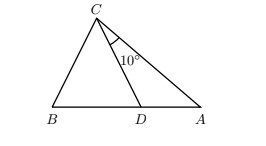
\includegraphics[scale=1]{ACImg1.jpg}
    \end{center}
\end{example}
\begin{soln}
    Como $\angle BCA=180-\angle CAB-\angle ABC=180-110=70^{\circ}$. Entonces $\angle BCD=\angle BCA-\angle DCA=60^{\circ}$, y como $DC=DB$ entonces $\angle DBC=\angle DCB=60^{\circ}$, asi que $\angle DCA=\angle DCB+\angle DBC=120$ y $\angle CAB=180-\angle ACD+\angle ADC=180-10-120=50^{\circ}$
\end{soln}

\subsection{Paralelas y opuestos por el vertice}
Estas son igualdades de \'angulos muy conocidas, no tengo mucho que agregar.
\begin{proposition}
    
    En esta imagen hay dos rectas paralelas y una recta que las intersecta, entonces los \'angulos rojos son iguales.
    \begin{center}
    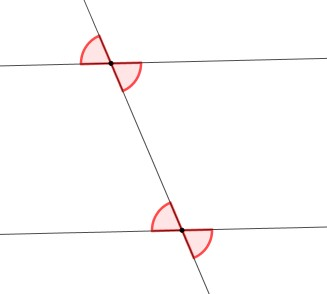
\includegraphics[scale=.5]{AC2.jpg}
    \end{center}
    A traves de un punto es opuestos por el vertice, a traves de las dos rectas paralelas es entre paralelas.
\end{proposition}

\subsection{Circulos}
Los circulos nos ayudan a mover muchos \'angulos, principalmente con lo siguiente.
\begin{theorem}
    [\'Angulos inscritos]
    Si el \'angulo $\angle ACB$ esta inscrito en el circulo (los 3 puntos estan en el circulo), entonces abre un arco de $2\angle ACB$.
    \begin{center}
        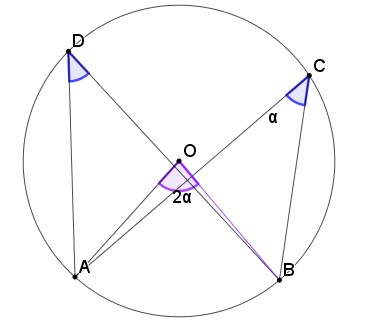
\includegraphics[scale=0.5]{AC3.jpg}
    \end{center}
\end{theorem}
Particularmente
\begin{theorem}
    Sea $M$ el punto medio del arco $AB$ que abre el \'angulo $\angle ACB$, entonces $CM$ es bisectriz de $\angle ACB$.
\end{theorem}
Esto sale aprovechando el isosceles que te da y moviendo los \'angulos con los arcos. \\
Ahora, estos \'angulos se suelen aprovechar mayormente con cierto tipo de cuadrilateros, los cuadrilateros ciclicos.
\begin{definition}
    Se dice que un cuadrilatero $ABCD$ es ciclico si y solo si $A,B,C,D$ estan en una misma circunferencia.
\end{definition}


Y entonces las siguientes tres condiciones son equivalentes en un cuadrilatero $ABCD$ (es decir, si una se cumple se cumplen todas y si una no se cumple ninguna se cumple). 
\begin{itemize}
    \item $ABCD$ es ciclico
    \item $\angle ABC+\angle CDA=180$
    \item $\angle ABD=\angle ACD$
\end{itemize}
En particular quiero enfatizar el uso de los \'angulos inscritos en los cuadrilateros ciclicos, ya que tienes muchos \'angulos que abren los mismos arcos y por lo tanto son iguales (En esto se usa el 3er punto).
\begin{example}
    Sea $ABCD$ un cuadrilatero ciclico. Sea F el punto medio del arco $AB$ que no contiene a $C$ ni a $D$. Las lineas $DF$ y $AC$ se intersecan en $P$ y las lineas $CF$ y $BD$ se intersecan en $Q$. Demuestra que $PQ$ y $AB$ son paralelas.
\end{example}
\begin{soln}
    \begin{center}
        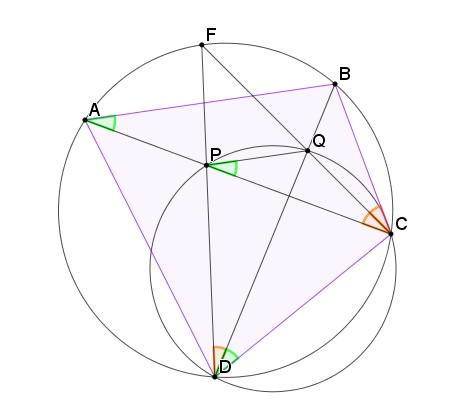
\includegraphics[scale=0.8]{Img5.jpg}
    \end{center}
    Como $F$ es el punto medio del arco $AB$ entonces $\angle BCF=\angle FCA$ y por lo tanto
    $$\angle QDP=\angle BDF=\angle BCF=\angle FCA=\angle QCP$$
    Por lo que $QPCD$ es ciclico y entonces 
    $$\angle CPQ=\angle CDQ=\angle CDB=\angle CAB$$
    Por lo que son paralelas.
\end{soln}
\begin{theorem}
     Si tienes un triangulo $ABC$ inscrito en un circulo $\omega$ con centro $O$ y un punto $P$ entonces estos 3 son equivalentes:
\begin{itemize}
    \item $PA$ es tangente a $\omega$
    \item $OA \perp PA$
    \item $\angle PAB=\angle ACB$
\end{itemize}
\end{theorem}


\subsection{H y 0}
    Si trazamos las alturas $AD,BE,CF$ y el ortocentro $H$ nos quedan los siguientes \'angulos (Mismo color es que son iguales).
    \begin{center}
        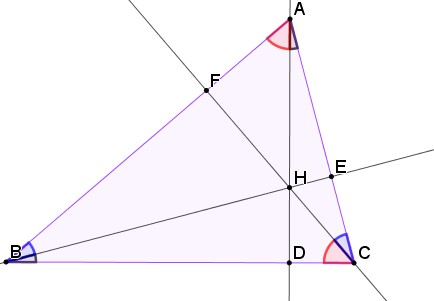
\includegraphics[scale=0.8]{AC6.jpg}
    \end{center}
    Esto por los distintos ciclicos que se forman por los \'angulos de 90 (Adem\'as dos angulos de 90 suman 180). \\
    Estos ciclicos son: 
    $$AEHF, CDHE, BFHD, AEDB, CDFA, BFEC$$
    Adem\'as estos nos dan que $H$ es el incentro de $DEF$. 
    \begin{definition}
        En un triangulo dos rectas se llaman isogonales si pasan por un vertice y son reflejadas respecto a la bisectriz de ese vertice. 
    \end{definition}
    \begin{theorem}
        En un triangulo $ABC$, se cumple que $AH, AO$ son isogonales.
    \end{theorem}
    \begin{proof}
        Se tiene que $\angle BAH=90-\angle B$ y adem\'as $\angle AOC=2\angle B$ y como $OA=OC$ entonces $\angle CAO=\frac{180-2\angle B}{2}=90-\angle B$, entonces como el \'angulo es el mismo son isogonales.
    \end{proof}
\subsection{Bisectrices}
    Si estamos pensando en \'angulos las bisectrices tienen sentido que aparezcan, ya que estas te dan igualdades en \'angulos. \\
    Ahora pensando mas en incentros y excentros ya que estos en base a dos bisectrices (ya sean internas o externas) te dan una tercera la cual puede ser de mucha ayuda. 

    \begin{example}
    Sea $ABC$ un triangulo acutangulo, sea $D$ el pie de altura desde $C$. La bisectriz de $\angle ABC$ intersecta $CD$ en $E$ e intersecta al circuncirculo $\omega$ de $ADE$ en $F$. Si $\angle ADF=45$ muestra que $CF$ es tangente a $\omega$.
    \end{example}
 
\subsection{Reflejar}
    Podemos reflejar principalmente sobre un punto o sobre una recta. \\
    Reflejar sobre un punto $P$ es agarrar todos los punto $X$ del plano y mandarlos al punto $X'$ tal que $P$ es el punto medio de $XX'$ (en otras palabras, tomas la distancia de $XP$ y usas la misma distancia pero en el lado contrario). \\
    Reflejar sobre una recta $l$ es agarrar todos los puntos $X$ del plano y mandarlos al punto $X'$ tales que $l$ es la mediatriz de $XX'$ (en otras palabras tomar la distancia a la recta y usarla pero en el lado contrario) \\
    Reflejar cumple que si reflejas dos veces es como si no hubieras hecho nada. \\
    Hacer reflexiones puede ser muy util en Angle Chasing para dos cosas, poder igualar \'angulos sabiendo que cierta parte del dibujo es el reflejo de otra parte del dibujo, o para crear puntos/trazos auxiliares con ciertas propiedades y que te pueden dar ciclicos, paralelas, u otro tipo de informaci\'on.  \\
    \begin{theorem}
    En un triangulo $ABC$ con ortocentro $H$, punto medio de $BC$ $M$, $X$ la reflexi\'on de $H$ sobre $BC$, $Y$ la reflexi\'on de $H$ sobre $M$. Se cumple que 
    $AY$ es diametro de el circuncirculo y que $X$ esta en el circuncirculo.
    \end{theorem}
    \begin{proof}
        .
        \begin{center}
         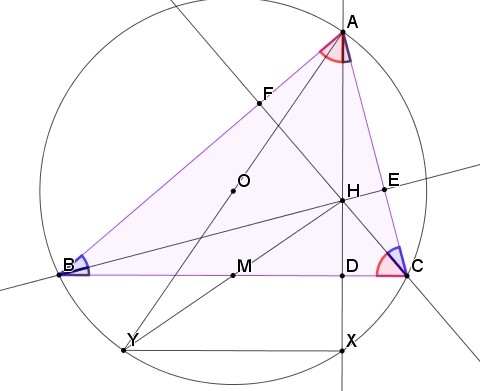
\includegraphics[scale=0.5]{AC7.jpg}
        \end{center}
        Se puede calcular que $\angle BHC=180-\angle A$ entonces $\angle BXC=180-\angle A$, asi que $BXCA$ es ciclico. \\
        Y como $MH=MY$ y $MB=MC$ entonces $HBYC$ es un paralelogramo y $\angle BYC=180-\angle A$ asi que $BYCA$ tambien es ciclico. \\
        Y como $MD || YX$ por tales, entonces $\angle YXA=\angle MDH=90$, entonces $AY$ es diametro.
    \end{proof}
    Como se acaba de mostrar una reflexi\'on muy util es reflejar sobre algun punto medio para obtener paralelogramos, otro ejemplo es:
    \begin{example}
        
    Sea $ABC$ un triángulo acutángulo con $AB \neq AC$, $M$ el punto medio de $BC$ y $H$ el
ortocentro de $ABC$. La circunferencia que pasa por $B$, $H$ y $C$ corta a la mediana $AM$ en
$N$. Muestra que $\angle ANH = 90^o$.
    
    \end{example}
    \begin{soln}
    \begin{center}
        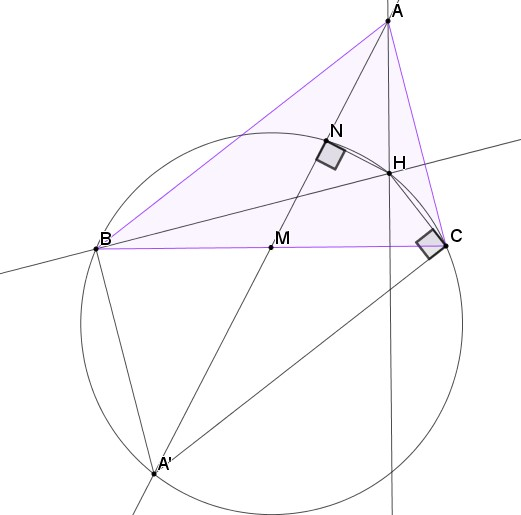
\includegraphics[scale=0.5]{AC5.jpg}
    \end{center}
        Sea $A'$ la reflexi\'on de $A$ sobre $M$, en particular $BACA'$ es un paralelogramo porque $MB=MC$ y $MA=MA'$. Entonces $\angle BA'C=\angle A$ y 
        $$\angle BHC =180-\angle HBC-\angle HCB=180-90+\angle C-90+\angle B=180-\angle A$$
        Por lo que $BHCA'$ es ciclico. Y como $\angle (HC, CA')=(HC,AB)=90$ por las paralelas, entonces el ciclico $NHCA'$ tiene diametro $A'H$ y $\angle A'NH=90$ y $\angle ANH=90$
    \end{soln}

    Otra reflexi\'on muy util en triangulos es reflejar sobre alguna bisectriz. 
    \begin{example}
        Sea $ABC$ un triangulo con circuncentro $O$ y ortocentro $H$. Prueba que $AO=AH$ si y solo si $\angle BAC=60$
    \end{example}
    \begin{soln}
    .
        \begin{center}
            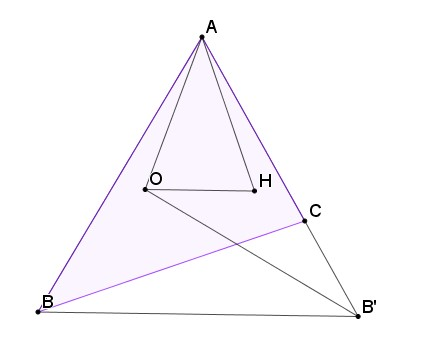
\includegraphics[scale=0.5]{Img16.jpg}
        \end{center}
        Si $AO=AH$ sucede que: \\
        Como $\angle BAO=\angle CAH$, entonces al reflejar $O$ sobre la bisectriz de $\angle BAC$ nos queda $H$, y digamos que al reflejar $B$ nos queda $B'$. Entonces 
        $$\angle (B'O, AB)=\angle (BH, AB')=90$$
        Asi que $B'$ esta en la mediatriz de $AB$ y entonces $AB=AB'=BB'$ generando un triangulo equilatero y el \'angulo de 60 necesario. 
        (El regreso es practicamente analogo.)
    \end{soln}
\newpage
\epigraph{Calificadores en decadencia ya ni holder saben}{Takumi}
\section{Problemas Parte 1}

\begin{problem}  En la siguiente figura $AD=BC$.¿Cuánto mide el ángulo $\angle DAC$?
\begin{center}
  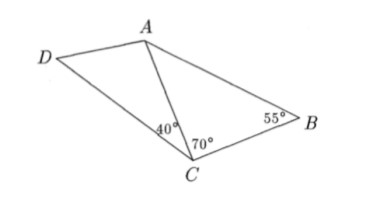
\includegraphics[scale=0.9]{I1.jpg}  
\end{center}


\end{problem}
\begin{problem}
    Demuestra que la suma de los angulos internos de un poligono de $n$ lados es $180(n-2)$
\end{problem}
\begin{problem}
    En la configuraci\'on del ortocentro demuestra que $\triangle AEF,BFD,CDE,ABC $ son semejantes entre si.
\end{problem}
\begin{problem}
    En la configuraci\'on del ortocentro demuestra que $H$ es el incentro de $DEF$.
\end{problem}
\begin{problem}
    Sea $P$ un punto dentro del circulo $\omega$, considera todas las cuerdas que contienen a $P$. Demuestra que todos sus puntos medios estan en un circulo.
\end{problem}

\begin{problem} 
En un triangulo $ABC$ se tiene la bisectriz $AD$ con $D$ en $BC$. Si se tiene que $AC=BC=AD$, determina el valor de 7 veces el angulo $\angle ACB$.
\end{problem}
\begin{problem}
    Sea $ABC$ un triangulo con circuncirculo $\omega$. Prueba que $AC \perp CB $ si y solo si $AB$ es diametro de $\omega$.
\end{problem}

\begin{problem}
Sea $ABCD$ y sea $BED$ un triangulo isosceles. ¿Cuánto mide el ángulo $\angle BCE$?.
\begin{center}
    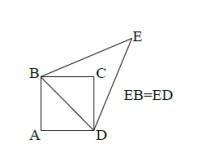
\includegraphics{I4.jpg}
\end{center}
\end{problem}

\begin{problem}
En la figura $ABCD$ es un cuadrado y $OBC$ es un triangulo equilatero. ¿Cuánto mide el ángulo $\angle OAC$?.
\begin{center}
    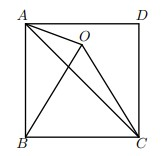
\includegraphics[]{I2.jpg}
\end{center}
\end{problem}

\begin{problem}
Si $I$ es el incentro del triangulo $ABC$ prueba que 
$$\angle BIC =90+\half \angle BAC$$
\end{problem}

\newpage
\section{Problemas Parte 2}
Los problemas no estan necesariamente en orden de dificultad. \\
Si resuelves al menos 6 problemas de esta parte dime y te mando la parte 3. 
\begin{problem}
    En la siguiente figura estan trazadas las bisectrices de los angulos interiores del cuadrilatero $ABCD$ las cuales se intersecan en $E,F,G,H$ demuestra que $EFGH$ es un cuadrilatero ciclico.
    \begin{center}
        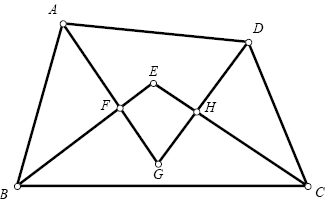
\includegraphics[scale=0.7]{I3.png}
    \end{center}
\end{problem}



\begin{problem}
 Sea $ABC$ un triangulo acutangulo con ortocentro $H$ y circuncentro $O$. Prueba que $\angle BAH=\angle CAO$.
\end{problem}
\begin{problem}
    Prueba que un trapecio es ciclico si y solo si es isosceles.
\end{problem}

\begin{problem}
    Tienes las dos tangentes $PA, PB$ a una circunferencia desde $P$, demuestra que $PA=PB$.
\end{problem}
\begin{problem}
    Sea $t$ una tangente por el vertice $C$ al circuncirculo de un triangulo $ABC$. Una recta $p$ paralela a $t$ intersecta $BC,AC$ en los puntos $D,E$. Demuestra que $A,B,D,E$ son conciclicos. 
\end{problem}

\begin{problem}
    Sea $ABC$ un triangulo. El incirculo de $ABC$ es tangente a $AB, AC$ en $D,E$. Sea $O$ el circuncentro de $BCI$. Demuestra que $\angle ODB=\angle OEC$
\end{problem}

\begin{problem}
    En un triangulo rectangulo $ABC$ con $\angle A=90, \angle C=30$. Sea $\omega$ el circulo que pasa por $A$ y es tangente a $BC$ en el punto medio. $\omega$ intersecta $AC$ en $N$ y al circuncirculo de $ABC$ en $M$. Prueba que $MN \perp BC$.
\end{problem}

\begin{problem} 
    Sea $ABCD$ un cuadrado y sea $Y$ un punto dentro de la diagonal $AC$ distinto del punto medio de $AC$. La recta perpendicular al segmento $BY$ que pasa por $Y$ corta a la recta $AD$ en $X$ y a la recta $CD$ en $Z$. Muestra que $AX=CZ$. 
\end{problem}
\begin{problem} 
    Sea $ABC$ un triangulo y sea $P$ cualquier punto en su circuncirculo. Sea $X,Y,Z$ los pies de altura desde $P$ hasta $BC,CA$ y $AB$. Prueba que los puntos $X,Y,Z$ son colineales.
\end{problem}

\begin{problem}
    Sea $I$ el incentro de un triangulo $ABC$ con $AB<AC$. La linea $AI$ intersecta el circuncirculo de $ABC$ en $D$. El circuncirculo de $CDI$ intersecta $BI$ de nuevo en $K$. Prueba que $BK=CK$.
\end{problem}


\end{document}